% Options for packages loaded elsewhere
\PassOptionsToPackage{unicode}{hyperref}
\PassOptionsToPackage{hyphens}{url}
%
\documentclass[
  english,
  doc,floatsintext]{apa6}
\usepackage{amsmath,amssymb}
\usepackage{lmodern}
\usepackage{iftex}
\ifPDFTeX
  \usepackage[T1]{fontenc}
  \usepackage[utf8]{inputenc}
  \usepackage{textcomp} % provide euro and other symbols
\else % if luatex or xetex
  \usepackage{unicode-math}
  \defaultfontfeatures{Scale=MatchLowercase}
  \defaultfontfeatures[\rmfamily]{Ligatures=TeX,Scale=1}
\fi
% Use upquote if available, for straight quotes in verbatim environments
\IfFileExists{upquote.sty}{\usepackage{upquote}}{}
\IfFileExists{microtype.sty}{% use microtype if available
  \usepackage[]{microtype}
  \UseMicrotypeSet[protrusion]{basicmath} % disable protrusion for tt fonts
}{}
\makeatletter
\@ifundefined{KOMAClassName}{% if non-KOMA class
  \IfFileExists{parskip.sty}{%
    \usepackage{parskip}
  }{% else
    \setlength{\parindent}{0pt}
    \setlength{\parskip}{6pt plus 2pt minus 1pt}}
}{% if KOMA class
  \KOMAoptions{parskip=half}}
\makeatother
\usepackage{xcolor}
\IfFileExists{xurl.sty}{\usepackage{xurl}}{} % add URL line breaks if available
\IfFileExists{bookmark.sty}{\usepackage{bookmark}}{\usepackage{hyperref}}
\hypersetup{
  pdftitle={Compre Report for Study Project on `Sports Analytics'},
  pdfauthor={Ahmed Thahir1},
  pdflang={en-EN},
  pdfkeywords={Sports Analytics, Causal Analysis, Machine Learning, Python, Statistics, Economics, Regression, Granger Causality, Time Series Data, Cross-Sectional Data},
  hidelinks,
  pdfcreator={LaTeX via pandoc}}
\urlstyle{same} % disable monospaced font for URLs
\usepackage{graphicx}
\makeatletter
\def\maxwidth{\ifdim\Gin@nat@width>\linewidth\linewidth\else\Gin@nat@width\fi}
\def\maxheight{\ifdim\Gin@nat@height>\textheight\textheight\else\Gin@nat@height\fi}
\makeatother
% Scale images if necessary, so that they will not overflow the page
% margins by default, and it is still possible to overwrite the defaults
% using explicit options in \includegraphics[width, height, ...]{}
\setkeys{Gin}{width=\maxwidth,height=\maxheight,keepaspectratio}
% Set default figure placement to htbp
\makeatletter
\def\fps@figure{htbp}
\makeatother
\setlength{\emergencystretch}{3em} % prevent overfull lines
\providecommand{\tightlist}{%
  \setlength{\itemsep}{0pt}\setlength{\parskip}{0pt}}
\setcounter{secnumdepth}{-\maxdimen} % remove section numbering
% Make \paragraph and \subparagraph free-standing
\ifx\paragraph\undefined\else
  \let\oldparagraph\paragraph
  \renewcommand{\paragraph}[1]{\oldparagraph{#1}\mbox{}}
\fi
\ifx\subparagraph\undefined\else
  \let\oldsubparagraph\subparagraph
  \renewcommand{\subparagraph}[1]{\oldsubparagraph{#1}\mbox{}}
\fi
\newlength{\cslhangindent}
\setlength{\cslhangindent}{1.5em}
\newlength{\csllabelwidth}
\setlength{\csllabelwidth}{3em}
\newlength{\cslentryspacingunit} % times entry-spacing
\setlength{\cslentryspacingunit}{\parskip}
\newenvironment{CSLReferences}[2] % #1 hanging-ident, #2 entry spacing
 {% don't indent paragraphs
  \setlength{\parindent}{0pt}
  % turn on hanging indent if param 1 is 1
  \ifodd #1
  \let\oldpar\par
  \def\par{\hangindent=\cslhangindent\oldpar}
  \fi
  % set entry spacing
  \setlength{\parskip}{#2\cslentryspacingunit}
 }%
 {}
\usepackage{calc}
\newcommand{\CSLBlock}[1]{#1\hfill\break}
\newcommand{\CSLLeftMargin}[1]{\parbox[t]{\csllabelwidth}{#1}}
\newcommand{\CSLRightInline}[1]{\parbox[t]{\linewidth - \csllabelwidth}{#1}\break}
\newcommand{\CSLIndent}[1]{\hspace{\cslhangindent}#1}
% Manuscript styling
\usepackage{upgreek}
\captionsetup{font=singlespacing,justification=justified}

% Table formatting
\usepackage{longtable}
\usepackage{lscape}
% \usepackage[counterclockwise]{rotating}   % Landscape page setup for large tables
\usepackage{multirow}		% Table styling
\usepackage{tabularx}		% Control Column width
\usepackage[flushleft]{threeparttable}	% Allows for three part tables with a specified notes section
\usepackage{threeparttablex}            % Lets threeparttable work with longtable

% Create new environments so endfloat can handle them
% \newenvironment{ltable}
%   {\begin{landscape}\centering\begin{threeparttable}}
%   {\end{threeparttable}\end{landscape}}
\newenvironment{lltable}{\begin{landscape}\centering\begin{ThreePartTable}}{\end{ThreePartTable}\end{landscape}}

% Enables adjusting longtable caption width to table width
% Solution found at http://golatex.de/longtable-mit-caption-so-breit-wie-die-tabelle-t15767.html
\makeatletter
\newcommand\LastLTentrywidth{1em}
\newlength\longtablewidth
\setlength{\longtablewidth}{1in}
\newcommand{\getlongtablewidth}{\begingroup \ifcsname LT@\roman{LT@tables}\endcsname \global\longtablewidth=0pt \renewcommand{\LT@entry}[2]{\global\advance\longtablewidth by ##2\relax\gdef\LastLTentrywidth{##2}}\@nameuse{LT@\roman{LT@tables}} \fi \endgroup}

% \setlength{\parindent}{0.5in}
% \setlength{\parskip}{0pt plus 0pt minus 0pt}

% \usepackage{etoolbox}
\makeatletter
\patchcmd{\HyOrg@maketitle}
  {\section{\normalfont\normalsize\abstractname}}
  {\section*{\normalfont\normalsize\abstractname}}
  {}{\typeout{Failed to patch abstract.}}
\patchcmd{\HyOrg@maketitle}
  {\section{\protect\normalfont{\@title}}}
  {\section*{\protect\normalfont{\@title}}}
  {}{\typeout{Failed to patch title.}}
\makeatother
\shorttitle{Sports Analytics}
\keywords{Sports Analytics, Causal Analysis, Machine Learning, Python, Statistics, Economics, Regression, Granger Causality, Time Series Data, Cross-Sectional Data}
\usepackage{csquotes}
\usepackage[titles]{tocloft}
\cftpagenumbersoff{figure}
\renewcommand{\cftfigpresnum}{\itshape\figurename\enspace}
\renewcommand{\cftfigaftersnum}{.\space}
\setlength{\cftfigindent}{0pt}
\setlength{\cftafterloftitleskip}{0pt}
\settowidth{\cftfignumwidth}{Figure 10.\qquad}
\cftpagenumbersoff{table}
\renewcommand{\cfttabpresnum}{\itshape\tablename\enspace}
\renewcommand{\cfttabaftersnum}{.\space}
\setlength{\cfttabindent}{0pt}
\setlength{\cftafterloftitleskip}{0pt}
\settowidth{\cfttabnumwidth}{Table 10.\qquad}
\usepackage{float} \usepackage{multirow}
\ifXeTeX
  % Load polyglossia as late as possible: uses bidi with RTL langages (e.g. Hebrew, Arabic)
  \usepackage{polyglossia}
  \setmainlanguage[]{english}
\else
  \usepackage[main=english]{babel}
% get rid of language-specific shorthands (see #6817):
\let\LanguageShortHands\languageshorthands
\def\languageshorthands#1{}
\fi
\ifLuaTeX
  \usepackage{selnolig}  % disable illegal ligatures
\fi

\title{Compre Report for Study Project on `Sports Analytics'}
\author{Ahmed Thahir\textsuperscript{1}}
\date{}


\affiliation{\vspace{0.5cm}\textsuperscript{1} BITS Pilani Dubai Campus}

\abstract{
Sports analytics is a field of study involved in understanding and improving sports performance of team(s) and player(s), using relevant data. It has been found that current research in Sports Analytics primarily focuses on prediction using statistical correlation, rather than making decisions using causation. My research proposes using causal inference to identify parameters that can improve a team/players' performance. Moreover, the idea of using economics principles for financial decisions such as player transfers has also been introduced here. Furthermore, a basic use-case of Granger Causality has also been implemented.
}



\begin{document}
\maketitle



\newpage
\pagenumbering{roman}

\hypertarget{acknowledgements}{%
\section{Acknowledgements}\label{acknowledgements}}

Firstly, I would like to thank Almighty God for giving me the strength, knowledge, ability and opportunity to take this project.

Secondly, I would like to thank my family and friends, who have always supported me in this journey of finding my true passion.

Thirdly, I would like to mention people who have inspired me. Mohammed Azharudin is the person who started it all - he sparked my interest in Computer Engineering. Dr.~Sartaj Rasool, my Economics professor, opened my eyes to the beautiful world of economics. A big thank you to all the teachers who have helped me get to the stage I am at right now.

Moreover, I would like to express my heartfelt gratitude to the Director of BITS Pilani, Dubai Campus, Prof.~Srinivasan Madapusi, who has ushered a new light on our college.

Lastly, I would like to thank my project supervisor, Dr.~Raja Muthalagu, for providing me with the opportunity of performing this project. His guidance and encouragement over the past few months has helped me learn and to be innovative.

\newpage
\tableofcontents

\newpage
\listoffigures
\listoftables

\newpage
\pagenumbering{arabic}

\hypertarget{chapter-1-introduction}{%
\section{Chapter 1: Introduction}\label{chapter-1-introduction}}

\hypertarget{authorization}{%
\subsection{Authorization}\label{authorization}}

This report for `Study Project on Sports Analytics' has been authorized by Dr.~Raja Muthalagu, HOD of Computer Science at BITS Pilani Dubai Campus, on 4\textsuperscript{th} April 2022.

\hypertarget{historical-background}{%
\subsection{Historical Background}\label{historical-background}}

Sports Analytics reached a global market size of \(\$ 2.5B\) in 2021. It has become widely-used by teams all over the world, with an expected market size of \(\$ 8.4 B\) by 2026. \protect\hyperlink{ref-SportsAnalyticsMarket}{{[}1{]}} Due to increasing competitiveness and limited resources, it has become essential to use data for optimization.

\hypertarget{objectives}{%
\subsection{Objectives}\label{objectives}}

\begin{itemize}
\tightlist
\item
  Identify parameters/factors which produce effective outcomes in sports.
\item
  The goal is not prediction, but to find causes.
\end{itemize}

\hypertarget{scope}{%
\subsection{Scope}\label{scope}}

\begin{itemize}
\tightlist
\item
  The report covers an outline of the research performed over the past few months for `Study Project on Sports Analytics'
\item
  The sport under this study is European Football.
\item
  Details not relevant to the topic in hand have been omitted
\end{itemize}

\hypertarget{limitations}{%
\subsection{Limitations}\label{limitations}}

\begin{itemize}
\tightlist
\item
  As this is a Study Project, the report only focuses on the learned concepts
\item
  The report does not go into depth into all details, as the field is quite vast
\item
  My proposed methods may be improvised, once I learn all the required concepts
\item
  Implementation of my proposed methods will be worked in the upcoming months
\end{itemize}

\hypertarget{methods-and-sources-of-data-collection}{%
\subsection{Methods and Sources of Data Collection}\label{methods-and-sources-of-data-collection}}

The main sources for research were online videos, articles, periodicals. Datasets were taken from open-access databases.

\hypertarget{report-review}{%
\subsection{Report Review}\label{report-review}}

Including the introduction, the report is divided into five chapters. Chapter-2 contains the \textbf{literature review} which highlights the existing research in this field. Chapter-3 is the \textbf{discussion}. Chapter-4 contains \textbf{implementation} of the existing research, to get an idea of statistical computing. Chapter-5 contains the \textbf{conclusion}, which sums up the discussions, insights and outlines the major issues faced.

\newpage

\hypertarget{chapter-2-theory}{%
\section{Chapter 2: Theory}\label{chapter-2-theory}}

This chapter highlights the major theoretical concepts that were come across during this study project. The references for this section are \protect\hyperlink{ref-chazan-pantzalisSportsAnalyticsAlgorithms2020}{{[}2{]}}--\protect\hyperlink{ref-FoundationsSportsAnalytics}{{[}4{]}}.

\hypertarget{definitions}{%
\subsection{Definitions}\label{definitions}}

This section highlights the major keywords and definitions relevant to this study.

\hypertarget{data-analytics}{%
\subsubsection{Data Analytics}\label{data-analytics}}

Data analytics is a field of study, which aims at obtaining useful insights using relevant data. Upon taking actions, further data is collected to verify the initial insights.

\hypertarget{sports-analytics}{%
\subsubsection{Sports Analytics}\label{sports-analytics}}

Sports analytics is a form of data analytics, involved in understanding and improving sports performance of team(s) and player(s).

\hypertarget{pythagorean-expectation} \propto\frac{x^2}{x^2 + y^2}
\]

where

\begin{itemize}
\tightlist
\item
  x = parameter scored
\item
  y = parameter conceded
\end{itemize}

\hypertarget{coefficient-of-determination}{%
\subsubsection{Coefficient of Determination}\label{coefficient-of-determination}}

It shows how well data fits within the regression. It is represented as \(R^2\). It has a range of \([0, 1]\). Higher the better.

\hypertarget{inflation}{%
\subsubsection{Inflation}\label{inflation}}

It is defined as the rate at which prices of commodities increase.

\hypertarget{cpi}{%
\subsubsection{CPI}\label{cpi}}

``The Consumer Price Index is a measure of the average change over time in the prices paid by urban consumers for a market basket of consumer goods and services''.\protect\hyperlink{ref-ConsumerPriceIndex}{{[}5{]}} It helps include the effect of inflation during analyses.

\hypertarget{opportunity-cost}{%
\subsubsection{Opportunity Cost}\label{opportunity-cost}}

It is defined as the real cost associated with any action. It is what you are sacrificing by doing a particular action, rather than t.

\hypertarget{types-of-data}{%
\subsection{Types of Data}\label{types-of-data}}

\hypertarget{cross-sectional}{%
\subsubsection{Cross-Sectional}\label{cross-sectional}}

Data that spans over various features, for the same time interval of interest.

\begin{table}[H]
  \begin{center}
  \begin{tabular}{|c|c|c|}
  \hline
  \textbf{Year} & \textbf{Company} & \textbf{Revenue} \\ \hline
  2015 & A       & 1K      \\ \hline
  2015 & B       & 2K      \\ \hline
  2015 & C       & 3K      \\ \hline
  \end{tabular}
  \end{center}
  
  \captionsetup{justification=centering}
  \caption{Cross-Sectional Data}
\end{table}

\hypertarget{time-series}{%
\subsubsection{Time Series}\label{time-series}}

Data that spans over various time intervals, for the same feature of interest.

\begin{table}[H]
  \begin{center}
  \begin{tabular}{|c|c|c|}
  \hline
  \textbf{Year} & \textbf{Company} & \textbf{Revenue} \\ \hline
  2015 & A       & 1K      \\ \hline
  2016 & A       & 2K      \\ \hline
  2017 & A       & 3K      \\ \hline
  \end{tabular}
  \end{center}
  
  \captionsetup{justification=centering}
  \caption{Time Series Data}
\end{table}

\hypertarget{panel}{%
\subsubsection{Panel}\label{panel}}

A combination of cross-sectional and time series data, spanning over various features and time intervals.

\begin{table}[H]
  \begin{center}
  \begin{tabular}{|c|c|c|}
  \hline
  \textbf{Year} & \textbf{Company} & \textbf{Revenue} \\ \hline
  2015 & A       & 1K      \\ \hline
  2015 & B       & 3K      \\ \hline
  2016 & A       & 2K      \\ \hline
  2016 & B       & 3K      \\ \hline
  2016 & C       & 1K      \\ \hline
  2017 & B       & 3K      \\ \hline
  2017 & C       & 3K      \\ \hline
  \end{tabular}
  \end{center}
  
  \captionsetup{justification=centering}
  \caption{Panel Data}
\end{table}

\hypertarget{statistics}{%
\subsection{Statistics}\label{statistics}}

Contrary to common understanding, Correlation \(\ne\) Causation. That is, just because 2 variables are correlated does not necessarily mean that one causes the other.

There are 3 levels of statistical computing

\begin{table}[H]
  \begin{center}
  \begin{tabular}{|c|c|c|}
  \hline
  \textbf{Level} & \textbf{Meaning} & \textbf{Purpose}                               \\ \hline
  Correlation      & Statistical relationship between two variables        & Prediction                            \\ \hline
  Causal Effect    & Relationship between a cause and its resulting effect & Making decisions on tested sample     \\ \hline
  Causal Mechanism & Understanding the reason for causal effect            & Making decisions on interested sample \\ \hline
  \end{tabular}
  \end{center}
  
  \captionsetup{justification=centering}
  \caption{Levels of Statistical Computing}
\end{table}

\hypertarget{prediction-methods}{%
\subsection{Prediction Methods}\label{prediction-methods}}

\begin{table}[H]
  \begin{center}
  \begin{tabular}{|c|c|}
  \hline
  \textbf{Type of Prediction} & \textbf{Range Interval} \\ \hline
  Classification     & $[0,1]$        \\ \hline
  Value              & Continuous     \\ \hline
  \end{tabular}
  \end{center}

  \captionsetup{justification=centering}
  \caption{Types of Prediction Models}
\end{table}

Consider \(h(x)\) to be hypothesis function (prediction). The following are the most commonly-used prediction models.

\hypertarget{linear-regression}{%
\subsubsection{Linear Regression}\label{linear-regression}}

A value prediction algorithm, which finds a best-fit straight line for the data.
\[
h(x) = a_0 + a_1 x
\]

\hypertarget{polynomial-regression}{%
\subsubsection{Polynomial Regression}\label{polynomial-regression}}

A value prediction algorithm, which finds a best-fit curve for the data.
\[
h(x) = a_0 + a_1 x + \dots + a_n x^n
\]

\hypertarget{logistic-regression}{%
\subsubsection{Logistic Regression}\label{logistic-regression}}

A classification algorithm, which finds a best-fit line to separate 2 categories of data. It incorporates a \emph{Sigmoid Function} \(g(z)\) that maps the output range as \([0, 1]\).
\[
\begin{aligned}
h(x) &= g(a_0 + a_1 x) \\
g(z) &= \frac1{ 1+e^{-z} }
\end{aligned}
\]

\hypertarget{decision-tree}{%
\subsubsection{Decision Tree}\label{decision-tree}}

A classification and value prediction algorithm that contains a tree-like structure of nodes, with conditions in each of them. It is very useful for conditional problems.

\hypertarget{random-forests}{%
\subsubsection{Random Forests}\label{random-forests}}

A classification and value prediction algorithm that contains a collection of decision trees. The final output is an averaged output of the trees.

\hypertarget{supported-vector-machines}{%
\subsubsection{Supported Vector Machines}\label{supported-vector-machines}}

A classification algorithm that tries to find a \emph{hyperplane}, that tries to maximize the margin between different categories of data.

\hypertarget{rubins-causal-model}{%
\subsection{Rubin's Causal Model}\label{rubins-causal-model}}

A model for causal inference, that depends on randomized testing to derive causality. It is widely used for deriving the effectiveness of treatments and drugs. Using a correct randomized experiment, the correlation obtained is equal to causal effect of the input.

`Treatment' refers to applying the input (1), and `no treatment' refers to not applying the input (0). Outcomes are the output with/without the treatment.

The average treatment effect - the true causal effect of an input - is the difference between the average outcome with and without the treatment. Averaging improves accuracy, as the input is a random variable.

However, as it depends on experimentation and the input can only be binary - 0/1, it is not always feasible. The preferred causal inference model is Judea-Pearl model which derives causality from observational data.

\hypertarget{gini-coeffiecent}{%
\subsection{Gini Coeffiecent}\label{gini-coeffiecent}}

Quantifies disparities/inequality in a distribution. It is mainly used for quantifying income disparities of various locations, communities, etc.

\[
\begin{aligned}
G
&=\frac{2}{n^{2} \bar{x}} \sum\limits_{i=1}^{n} i\left(x_{i}-\bar{x}\right) \\
&=\frac{\sum\limits_{i=1}^{n}(2 i-n-1) x_{i}}{n \sum\limits_{i=1}^{n} x_{i}}
\end{aligned}
\]

\hypertarget{hypothesis-testing}{%
\subsection{Hypothesis Testing}\label{hypothesis-testing}}

A statistical tool involving a null hypothesis and an alternate hypothesis to determine validity of a hypothesis.

\hypertarget{p-value}{%
\subsubsection{p-Value}\label{p-value}}

It is the probability of the null hypothesis being true.

\hypertarget{statistical-significance}{%
\subsubsection{Statistical Significance}\label{statistical-significance}}

A statistical test is said to be significant, if it has a p-Value of \(p \le 0.05\).

\hypertarget{granger-causality}{%
\subsection{Granger Causality}\label{granger-causality}}

A model to determine if one time series affects another. It helps determine direction of causality, when there is a 2-way correlation. The past values of \(x\) are tested to determine if they have a statistically significant effect on the current value of \(y\), taking past values of \(x\) as regressors. However, it may \textbf{not always} give true causality.

\[
y_t = a + b y_{t-1} + c x_{t-1}
\]

\begin{itemize}
\tightlist
\item
  if \(c \ne 0\) , then \(x\) \textbf{granger causes} \(y\)
\item
  \(t\) and \(t-1\) are not necessarily years; it just denotes a time period
\end{itemize}

\hypertarget{implementation}{%
\subsection{Implementation}\label{implementation}}

The following are few of the major tools that I will be using for my research.

\begin{table}[H]
  \begin{center}
  \begin{tabular}{|c|c|}
  \hline
  \textbf{Purpose}                   & \textbf{Tool}    \\ \hline
  Programming Language               & Python           \\ \hline
  Dataframes Library                 & Pandas           \\ \hline
  Plotting Library                   & Matplotlib       \\ \hline
  Prediction Library                 & SciKit-Learn     \\ \hline
  Math Library                       & Numpy            \\ \hline
  Granger Causality Library          & Statsmodel       \\ \hline
  Integrated Development Environment & Jupyter Notebook \\ \hline
  \end{tabular}
  \end{center}
  
  \captionsetup{justification=centering}
  \caption{Tools used}
\end{table}

Python is the chosen programming language, as it is

\begin{enumerate}
\def\labelenumi{\arabic{enumi}.}
\tightlist
\item
  free
\item
  open source
\item
  easy to learn
\item
  widely-used
\item
  easy to collaborate
\end{enumerate}

\newpage

\hypertarget{chapter-3-literature-review}{%
\section{Chapter 3: Literature Review}\label{chapter-3-literature-review}}

\hypertarget{current-research}{%
\subsection{Current Research}\label{current-research}}

The main reference paper for my research is . It provided a comprehensive explanation of Sports Analytics.

Sports data can be in different forms - qualitative/quantitative or structured/unstructured. This data could include player actions, spatio-temporal data, biographical data, scouting reports, etc. Sports analytics involves collecting and analyzing this data in order to gain insights. \protect\hyperlink{ref-bhatnagarSystematicReviewSports2019}{{[}6{]}}

\protect\hyperlink{ref-dixonModellingAssociationFootball1997}{{[}7{]}} predicted the winner of a game, using a Poisson Distribution to predict the goals scored by each team. \protect\hyperlink{ref-maoIdentifyingKeysWin2016}{{[}8{]}} created a model to predict match outcome, using logistic regression. \protect\hyperlink{ref-kampakisUsingTwitterPredict}{{[}9{]}} used numerous machine learning algorithms on n-grams (a specific sequence of letters/words) to predict match outcomes. \protect\hyperlink{ref-broichStatisticalAnalysisFirst2014}{{[}10{]}} concluded that that shot efficiency is more important than the number of shots; number of passes and ball contacts are also important factors; the distance covered was not found to be important. \protect\hyperlink{ref-ruiz-ruizAnalysisEntriesPenalty2013}{{[}11{]}} analyzed the 2006 World Cup and found that winning teams enter the opponent's penalty area more often. \protect\hyperlink{ref-ruiz-ruizAnalysisEntriesPenalty2013}{{[}11{]}} analyzed the 2006 World Cup and found that winning teams hardly allowed opponents enter their penalty area.

\protect\hyperlink{ref-armatasEVALUATIONGOALSSCORED2009}{{[}12{]}} found that there are more second half goals than in the first half; moreover, the probability of scoring increases with time. \protect\hyperlink{ref-DIFFERENCESOFFENSIVEACTIONS}{{[}13{]}} found that top teams are more efficient and score more goals from within the penalty area, inferred to be due to tactical superiority; another differentiator between top teams and other teams is the number of key passes (passes that lead to a goal scoring opportunity). \protect\hyperlink{ref-evangelosWinnersLosersTop}{{[}14{]}} compared one-sided games with competitive ones; they found that one-sided winners had much better possession \%, ``one-v-one'' duels, number of passes, shots, shots on target, and shooting accuracy; but these were inapplicable close range games. \protect\hyperlink{ref-hughesAnalysisPassingSequences2005}{{[}15{]}} analyzed two different FIFA World Cups and found that were more goals scored from passing sequences that were longer rather than shorter; however, when the number of passes gets too large, more attempts were required to score a goal.

\protect\hyperlink{ref-chazan-pantzalisSportsAnalyticsAlgorithms2020}{{[}2{]}} created a binary classification model to predict how each team of various European Leagues would perform, using numerous parameters such as previous year position, wins, draws, losses, net transfer expenditure, etc. Moreover, it focused on player performance prediction, with a focus on central defenders. Various features such as passing, heading, aggression were obtained from the game \emph{Football Manager}. These were used to predict match rating of players. The best predictors were found to be interceptions, clearances, jumping reach and strength.

Finally, \protect\hyperlink{ref-dobsonPerformanceRevenueProfessional1998}{{[}16{]}} took a different approach. It performed a \emph{Granger causality test} to find that ``the influence of lagged revenue on current performance is greater than the influence of lagged performance on current revenue''. However, despite this research highlighting some form of causality, trying to improve performance through increasing revenue isn't feasible, as it is not an easily controllable parameter.

\hypertarget{gaps}{%
\subsection{Gaps}\label{gaps}}

\begin{enumerate}
\def\labelenumi{\arabic{enumi}.}
\item
  Current research mainly focuses on prediction
\item
  Over-reliance on correlation

  Correlation is useful for making predictions, but is insufficient for making effective decisions
\item
  Lack of causal inference

  Decisions without casual understanding may prove to be costly, as they may \textbf{not produce} efficient outcomes
\item
  Financial values are in absolute terms, rather than relative terms

  This is not accurate, as \(€ 50\rm{M}\) was much more valuable 10 years ago compared to present-day, due to inflation.
\end{enumerate}

\newpage

\hypertarget{chapter-4-my-research}{%
\section{Chapter 4: My Research}\label{chapter-4-my-research}}

The following are the insights I obtained when doing this study project, that were worth mentioning.

\hypertarget{causal-inference}{%
\subsection{Causal Inference}\label{causal-inference}}

Correlation between Win\% of a team and a team's number of passes does \textbf{not} necessarily imply that passing more during games will lead to higher Win\%. The same goes to other parameters such as possession percentage, passing accuracy, etc.

The best approach to identify effective parameters would be to use causality tests, and hence obtain true causes of improved performance for a team/player. These effective parameters may vary from team to team, as each team differs in its ambitions and style of play.

\hypertarget{economics}{%
\subsection{Economics}\label{economics}}

When analyzing the cost of buying a player, economic principles such as correcting values for inflation and opportunity cost analysis may be used. This will give a more holistic understanding of whether or not a player is worth buying.

A point to note is that the inflation within the football transfer market has been much higher than the consumer sector. Players that would've cost around \(€ 30M\) few years ago now cost around \(€ 80M\). This is due to large transfers made by big clubs for players, such as \emph{Neymar Jr.} in 2017 - costing Paris Saint-Germain around \(€ 222M\). Moreover, there has been a sudden influx of investments in the footballing world, thereby resulting in clubs demanding higher transfer fees to sell their players.

\hypertarget{implementation-1}{%
\subsection{Implementation}\label{implementation-1}}

A basic implementation was performed to learn using Python for statistical computing. The codes are available on the \href{https://github.com/AhmedThahir/StudyProject\#implementations}{GitHub repository} for this project.

\hypertarget{english-premier-league-predictor}{%
\subsubsection{English Premier League Predictor}\label{english-premier-league-predictor}}

This implementation tries to predict the 2nd half win\% of a team using data from the first half of the season. Using Pythagorean Expectation gave better results, as the correlation and \(R^2\) value was higher. Referred to \protect\hyperlink{ref-FoundationsSportsAnalytics}{{[}4{]}}

\begin{table}[H]
  \begin{center}
  \begin{tabular}{|c|c|c|}
  \hline
  \textbf{2nd Half Win\% predicted using 1st Half} & \textbf{$R^2$} & \textbf{Correlation} \\ \hline
  Win\%                                            & 0.572          & 0.757                \\ \hline
  Pythagorean Expectation                          & 0.633          & 0.796                \\ \hline
  \end{tabular}
  \end{center}
  
  \captionsetup{justification=centering}
  \caption{Win \% Prediction}
\end{table}

\begin{figure}[H]
  \begin{center}
  \includegraphics[width=0.9\linewidth, height=6cm]{assets/win.png}
  \end{center}
  
  \captionsetup{justification=centering}
  \caption{Win \%}
\end{figure}

\begin{figure}[H]
  \begin{center}
  \includegraphics[width=0.9\linewidth, height=6cm]{assets/pythagorean.png}
  \end{center}
  
  \captionsetup{justification=centering}
  \caption{Pythagorean}
\end{figure}

\hypertarget{fifa21-player-rating}{%
\subsubsection{FIFA21 Player Rating}\label{fifa21-player-rating}}

This implementation aims at predicting players' FIFA21 (an official football game) rating using their market value. An attempt at including the effect of inflation using CPI failed. Referred to \protect\hyperlink{ref-chazan-pantzalisSportsAnalyticsAlgorithms2020}{{[}2{]}}

\begin{figure}[H]
  \begin{center}
  \includegraphics[width=0.9\linewidth, height=6cm]{assets/Overall vs Value.png}
  \end{center}
  
  \captionsetup{justification=centering}
  \caption{Rating vs Value}
  \end{figure}

\begin{figure}[H]
  \begin{center}
  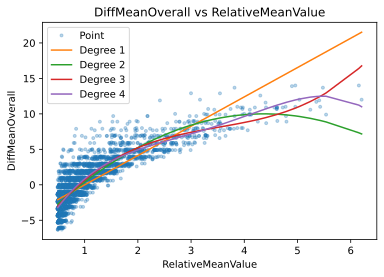
\includegraphics[width=0.9\linewidth, height=6cm]{assets/DiffMeanOverall vs RelativeMeanValue.png}
  \end{center}
  
  \captionsetup{justification=centering}
  \caption{Corrected using CPI and Mean Value}
\end{figure}

\hypertarget{inferences}{%
\paragraph{Inferences}\label{inferences}}

\begin{table}
  \begin{center}
  \begin{tabular}{|c|c|c|}
  \hline
  \textbf{Method} & \textbf{Degree} & \textbf{$R^2$ Value} \\ \hline
  \multicolumn{1}{|c|}{\multirow{4}{*}{Uncorrected}} & 1      & 0.5974      \\ \cline{2-3} 
  \multicolumn{1}{|c|}{}                             & 2      & 0.7076      \\ \cline{2-3} 
  \multicolumn{1}{|c|}{}                             & 3      & 0.7308      \\ \cline{2-3} 
  \multicolumn{1}{|c|}{}                             & 4      & 0.6696      \\ \hline
  \multirow{4}{*}{Corrected}                         & 1      & 0.6157      \\ \cline{2-3} 
                                                     & 2      & 0.7204      \\ \cline{2-3} 
                                                     & 3      & 0.7413      \\ \cline{2-3} 
                                                     & 4      & 0.7476      \\ \hline
  \end{tabular}
  \end{center}
  
  \captionsetup{justification=centering}
  \caption{Corrected using CPI and Mean Value}
\end{table}

\begin{itemize}
\tightlist
\item
  Only CPI is not enough to include the hyper inflation in football. CPI only shows an inflation of around 5\%; hyper-inflation is much higher than that. Hence, getting the deviation from the average transfer value of each year may provide a better result.
\item
  Relationship is only satisfied for players with value \(\ge 1M\). This \textbf{could} mean that there are many good under-valued players.
\item
  Corrected Degree 3\&4 Regression gave the best-fit. However, due to over-fitting, it has a downward slope at the end; hence, it is to be rejected.
\end{itemize}

\hypertarget{granger-causality-test-of-cristiano-ronaldos-market-value-performance-and-age}{%
\subsubsection{Granger Causality test of Cristiano Ronaldo's Market Value, Performance, and Age}\label{granger-causality-test-of-cristiano-ronaldos-market-value-performance-and-age}}

Hypothesis: Market Value is a function of previous year's performance and age.

\[
\begin{aligned}
V &\propto P \\
V & \propto \frac{1}{A} \\
V &= a V_{t-1} + b x_{t-1} \\
x &= \text{Goals} + \text{Assists} - \text{Age}
\end{aligned}
\]

The base/`zero' value of every player must be their initial value, as every player starts off from a different initial value. This is not just restricted to talent/skill, due to factors such as nationality. Moreover, it helps accommodate the market value of a player who started off with a high value won't really go \(< 1M\).

\begin{figure}[H]
  \begin{center}
  \includegraphics[width=0.9\linewidth, height=6cm]{assets/Goal_Contributions vs Mean_Value_Diff_From_First.png}
  \end{center}
  
  \captionsetup{justification=centering}
  \caption{Granger Causality test of Goal Contributions as a function of Market Value}
\end{figure}

\begin{figure}[H]
  \begin{center}
  \includegraphics[width=0.9\linewidth, height=6cm]{assets/Mean_Value_Diff_From_First vs Goal_Contributions.png}
  \end{center}
  
  \captionsetup{justification=centering}
  \caption{Granger Causality test of Market Value as a function of Goal Contributions}
\end{figure}

\begin{figure}[H]
  \begin{center}
  \includegraphics[width=0.9\linewidth, height=6cm]{assets/Mean_Value_Diff_From_First vs Input.png}
  \end{center}
  
  \captionsetup{justification=centering}
  \caption{Granger Causality test of Market Value as a function of Goal Contributions and Age}
\end{figure}

\hypertarget{inferences-1}{%
\paragraph{Inferences}\label{inferences-1}}

\begin{table}[H]
  \begin{center}
  \begin{tabular}{|c|c|c|c|}
  \hline
  \textbf{Prediction}                             & \textbf{Predictor}             & \textbf{p-Value} & Significant \\ \hline
  Goal\_Contributions                             & Mean\_Value\_Diff\_From\_First & 0.8667           & N          \\ \hline
  \multirow{2}{*}{Mean\_Value\_Diff\_From\_First} & Goal\_Contributions            & 0.0491           & Y           \\ \cline{2-4} 
                                                  & Goals\_Contributions - Age     & 0.0068           & Y           \\ \hline
  \end{tabular}
  \end{center}
  
  \captionsetup{justification=centering}
  \caption{Granger Causality test of Cristiano Ronaldo's Market Value, Performance, and Age}
\end{table}

\newpage

\hypertarget{chapter-5-conclusion}{%
\section{Chapter 5: Conclusion}\label{chapter-5-conclusion}}

There is clearly a lot of scope for sports analytics. Current research only focuses on prediction using correlation. However, this report highlighted the dangers of relying on statistical correlation. Causal inference is crucial for taking decisions that improve efficiency and avoid costly errors.

\hypertarget{concepts-to-learn}{%
\subsection{Concepts to Learn}\label{concepts-to-learn}}

To progress with my research, the next steps would be to learn

\begin{itemize}
\tightlist
\item
  Judea Pearl Causality Model
\item
  when to implement each prediction model
\item
  handling panel data
\end{itemize}

\hypertarget{possible-future-work}{%
\subsection{Possible Future Work}\label{possible-future-work}}

\begin{itemize}
\tightlist
\item
  Forecasting performance of player in the next season
\item
  Determining if a player would be a good purchase
\item
  Determining if collection of players with large variety of experience would perform better than a collection with the same experience, using Gini-Coefficient.
\end{itemize}

\newpage

\hypertarget{bibliography}{%
\section{Bibliography}\label{bibliography}}

\hypertarget{refs}{}
\begin{CSLReferences}{0}{0}
\leavevmode\vadjust pre{\hypertarget{ref-SportsAnalyticsMarket}{}}%
\CSLLeftMargin{{[}1{]} }
\CSLRightInline{{``Sports {Analytics Market} with {COVID-19 Impact Analysis} by {Component}, {Application}, {Deployment Mode}, {Organization Size}, {Industry Vertical And Region} - {Global Forecast} to 2026.''} https://www.reportlinker.com/p03825782/Sports-Analytics-Market-by-Type-by-Applications-by-Deployment-Type-by-Region-Global-Forecast-to.html?utm\_source=GNW.}

\leavevmode\vadjust pre{\hypertarget{ref-chazan-pantzalisSportsAnalyticsAlgorithms2020}{}}%
\CSLLeftMargin{{[}2{]} }
\CSLRightInline{V. Chazan - Pantzalis, {``Sports {Analytics Algorithms} for {Performance Prediction},''} Jun. 2020.}

\leavevmode\vadjust pre{\hypertarget{ref-ModernDataAnalysis}{}}%
\CSLLeftMargin{{[}3{]} }
\CSLRightInline{{``Modern {Data Analysis} for {Economics},''} \emph{Modern Data Analysis for Economics}. http://jiamingmao.github.io/data-analysis/.}

\leavevmode\vadjust pre{\hypertarget{ref-FoundationsSportsAnalytics}{}}%
\CSLLeftMargin{{[}4{]} }
\CSLRightInline{{``Foundations of {Sports Analytics}: {Data}, {Representation}, and {Models} in {Sports} \textbar{} {Coursera}.''} https://www.coursera.org/learn/foundations-sports-analytics.}

\leavevmode\vadjust pre{\hypertarget{ref-ConsumerPriceIndex}{}}%
\CSLLeftMargin{{[}5{]} }
\CSLRightInline{{``Consumer {Price Index} ({CPI}),''} \emph{Investopedia}. https://www.investopedia.com/terms/c/consumerpriceindex.asp.}

\leavevmode\vadjust pre{\hypertarget{ref-bhatnagarSystematicReviewSports2019}{}}%
\CSLLeftMargin{{[}6{]} }
\CSLRightInline{R. Bhatnagar and M. Babbar, \emph{A systematic review of sports analytics}. 2019.}

\leavevmode\vadjust pre{\hypertarget{ref-dixonModellingAssociationFootball1997}{}}%
\CSLLeftMargin{{[}7{]} }
\CSLRightInline{M. J. Dixon and S. G. Coles, {``Modelling {Association Football Scores} and {Inefficiencies} in the {Football Betting Market},''} \emph{Journal of the Royal Statistical Society: Series C (Applied Statistics)}, vol. 46, no. 2, pp. 265--280, Jan. 1997, doi: \href{https://doi.org/10.1111/1467-9876.00065}{10.1111/1467-9876.00065}.}

\leavevmode\vadjust pre{\hypertarget{ref-maoIdentifyingKeysWin2016}{}}%
\CSLLeftMargin{{[}8{]} }
\CSLRightInline{L. Mao, Z. Peng, H. Liu, and M.-A. Gómez, {``Identifying keys to win in the {Chinese} professional soccer league,''} \emph{International Journal of Performance Analysis in Sport}, vol. 16, no. 3, pp. 935--947, Dec. 2016, doi: \href{https://doi.org/10.1080/24748668.2016.11868940}{10.1080/24748668.2016.11868940}.}

\leavevmode\vadjust pre{\hypertarget{ref-kampakisUsingTwitterPredict}{}}%
\CSLLeftMargin{{[}9{]} }
\CSLRightInline{S. Kampakis and A. Adamides, {``Using {Twitter} to predict football outcomes,''} p. 10.}

\leavevmode\vadjust pre{\hypertarget{ref-broichStatisticalAnalysisFirst2014}{}}%
\CSLLeftMargin{{[}10{]} }
\CSLRightInline{H. Broich, J. Mester, and F. Seifriz, {``Statistical {Analysis} for the {First Bundesliga} in the {Current Soccer Season},''} p. 8, 2014.}

\leavevmode\vadjust pre{\hypertarget{ref-ruiz-ruizAnalysisEntriesPenalty2013}{}}%
\CSLLeftMargin{{[}11{]} }
\CSLRightInline{C. Ruiz-Ruiz, L. Fradua, Á. Fernández-GarcÍa, and A. Zubillaga, {``Analysis of entries into the penalty area as a performance indicator in soccer,''} \emph{European Journal of Sport Science}, vol. 13, no. 3, pp. 241--248, May 2013, doi: \href{https://doi.org/10.1080/17461391.2011.606834}{10.1080/17461391.2011.606834}.}

\leavevmode\vadjust pre{\hypertarget{ref-armatasEVALUATIONGOALSSCORED2009}{}}%
\CSLLeftMargin{{[}12{]} }
\CSLRightInline{V. Armatas, A. Yiannakos, S. Papadopoulou, and D. Skoufas, {``{EVALUATION OF GOALS SCORED IN TOP RANKING SOCCER MATCHES}: {GREEK} " {SUPERLEAGUE} " 2006-07,''} \emph{Serbian Journal of Sports Sciences}, vol. 3, pp. 39--43, Feb. 2009.}

\leavevmode\vadjust pre{\hypertarget{ref-DIFFERENCESOFFENSIVEACTIONS}{}}%
\CSLLeftMargin{{[}13{]} }
\CSLRightInline{{``{DIFFERENCES IN OFFENSIVE ACTIONS BETWEEN TOP AND LAST TEAMS IN GREEK FIRST SOCCER DIVISION}. {A RETROSPECTIVE STUDY} 1998-2008.''}}

\leavevmode\vadjust pre{\hypertarget{ref-evangelosWinnersLosersTop}{}}%
\CSLLeftMargin{{[}14{]} }
\CSLRightInline{B. Evangelos, G. Aristotelis, G. Ioannis, K. Stergios, and A. Foteini, {``Winners and losers in top level soccer. {How} do they differ?''} p. 8.}

\leavevmode\vadjust pre{\hypertarget{ref-hughesAnalysisPassingSequences2005}{}}%
\CSLLeftMargin{{[}15{]} }
\CSLRightInline{M. Hughes and I. Franks, {``Analysis of passing sequences, shots and goals in soccer,''} \emph{Journal of Sports Sciences}, vol. 23, no. 5, pp. 509--514, May 2005, doi: \href{https://doi.org/10.1080/02640410410001716779}{10.1080/02640410410001716779}.}

\leavevmode\vadjust pre{\hypertarget{ref-dobsonPerformanceRevenueProfessional1998}{}}%
\CSLLeftMargin{{[}16{]} }
\CSLRightInline{S. M. Dobson and J. A. Goddard, {``Performance and revenue in professional league football: Evidence from {Granger} causality tests,''} \emph{Applied Economics}, vol. 30, no. 12, pp. 1641--1651, Dec. 1998, doi: \href{https://doi.org/10.1080/000368498324715}{10.1080/000368498324715}.}

\end{CSLReferences}


\clearpage
\renewcommand{\listfigurename}{Figure captions}
\listoffigures
\clearpage
\renewcommand{\listtablename}{Table captions}
\listoftables

\end{document}
